\section{XML引论}

\begin{frame}{CH1 XML引论}
\begin{figure}
    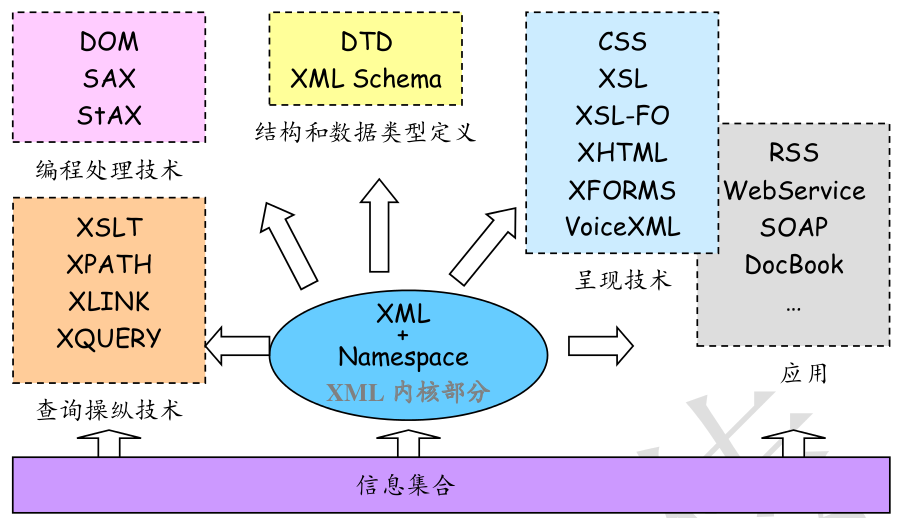
\includegraphics[width=0.9\textwidth]{figure/overview.png}
\end{figure}
\end{frame}

\begin{frame}[fragile]{目录}
\begin{easylist} \easyitem
& XML的起源
& XML的设计目标与特点
& XML技术体系
& XML的应用与发展
& XML相关工具
\end{easylist}
\end{frame}

\subsection{1.1 XML的起源}

\begin{frame}{1.1 XML的起源}
\begin{enumerate}
\item 标记起源
\item 过程标记:RTF
\item 通用编码:TEX
\item SGML
\item XML
\end{enumerate}
\end{frame}

\begin{frame}{标记起源}
\begin{itemize}
\item 标记语言(Markup Language)起源于传统印刷
\item  计算机中的电子标记(WPS、OpenOffice……)
\item 定义: 
\begin{shaded}标记语言就是一种用来给文本添加“格式标注”以指明文档中文本编排格式的语言,一般由定义文档格式的一些规定代码和控制标记组成。\end{shaded}
\end{itemize}
\end{frame}

\begin{frame}{过程标记}
\par 以微软开发的富文本格式 \framebox{RTF: Rich Text Format}为典型代表:
\begin{exampleblock} {例子}
	\par 用Word输入如下文字,并保存为rtf类型:
	\par {\color{red}XML} and RTF!
	\par 用记事本打开保存的文件,查看其文本内容
\end{exampleblock}
\end{frame}

\begin{frame}[fragile]{通用编码}
\par 以\framebox{TeX}为典型代表,例如以下代码片段:
\begin{exampleblock}{TeX示例}
  \begin{lstlisting}[tabsize=8,language=TeX]
  \noindent Tian Xia\par
  \noindent Information Resource Management\par
  \noindent Renmin University of China\par
  \smallskip
  This is a book about XML. It you have some problems, you can concat us directly.\par
  \bye
  \end{lstlisting}
\end{exampleblock}
\end{frame}


\begin{frame}[fragile]{SGML}
\par SGML(Standard Generalized Markup Language), 即标准通用标记语言, 是一种定义电子文档结构和描述其内容的国际标准语言, 早在 Web 发明之前 SGML 就已存在。由IBM的Goldfarb、Mosher 和 Lorie创造。
\par 是HTML、DocBook、XML等新标记语言的基础
\end{frame}


\begin{frame}[fragile, allowframebreaks]{HTML}
\par 1989 年由欧洲量子实验室的研究人员 Tim Berners Lee 在 SGML 的基础上开发的一个简化子集。
\begin{exampleblock}{HTML示例}
  \begin{lstlisting}[tabsize=8,language=HTML]
<html>
    <head>
        <title>HTML网页测试</title>
    </head>
    <body>
        <h1>简单的HTML</h1>
        <p>我的<font color="red">测试网页!</font></p>
    </body>
</html>
  \end{lstlisting}
\end{exampleblock}

\newpage
\par HTML本质上是通过标记的方式,以纯文本形式对网页进行描述,而对标记的解释则由浏览器执行,如现在流行的 IE (Internet Explorer)浏览器、 FireFox 浏览器、 Opera 浏览器等。浏览器读取网页源代码,即 HTML 标记文本,并通过渲染呈现给用户,就形成了用户最终看到的网页。
\begin{exampleblock}{HTML缺点}
\begin{itemize} 
\item 标记固定
\item 标记侧重于如何显示信息,缺乏对数据内容含义的表达能力
\item 缺乏严格的结构要求
\end{itemize}
\end{exampleblock}
\end{frame}


\begin{frame}[fragile, allowframebreaks]{XML}
\par W3C设计,删除了 SGML 中所有不必要的组件, 保留了 SGML 的基本原理: 标记用于描述文档结构; 模型必须与文档相关联。并注重简单性原则。
\par XML示例文档内容:
\begin{lstlisting}[tabsize=8,language=XML]
<?xml version="1.0" encoding="gb2312"?>
<?xml-stylesheet type="text/xsl" href="1-5.xsl"?>
<books>
    <book isbn="7-302-02368-9">
        <title>数据结构</title>
        <author>严蔚敏,吴伟民</author>
        <publisher>清华大学出版社</publisher>
        <price>22.0</price>
    </book>
</books>
\end{lstlisting}

\par XSLT示例文档内容:
\begin{lstlisting}[tabsize=8, basicstyle=\small\tt, language=XML]
<?xml version="1.0" encoding="gb2312"?>
<xsl:stylesheet version="1.0" xmlns:xsl="http://www.w3.org/1999/XSL/Transform">
    <xsl:template match="/">
        <html>
            <head><title>这是图书的呈现样式结果</title></head>
            <body>
                <table border="1">
                <tr>
                    <th>书名 </th>
                    <th>作者 </th>
                    <th>出版社 </th>
                    <th>价格 </th>						
                </tr>					
                <tr>
                    <td><xsl:value-of select="books/book/title"/></td>
                    <td><xsl:value-of select="books/book/author"/></td>
                    <td><xsl:value-of select="books/book/publisher"/></td>
                    <td><xsl:value-of select="books/book/price"/></td>						
                </tr>
                </table>
            </body>
        </html>
    </xsl:template>
</xsl:stylesheet>
\end{lstlisting}

\par {\color{red}用浏览器打开XML文档,查看效果}
\end{frame}


\begin{frame}[fragile]{SGML、HTML 与 XML 的关系}
\begin{figure}
	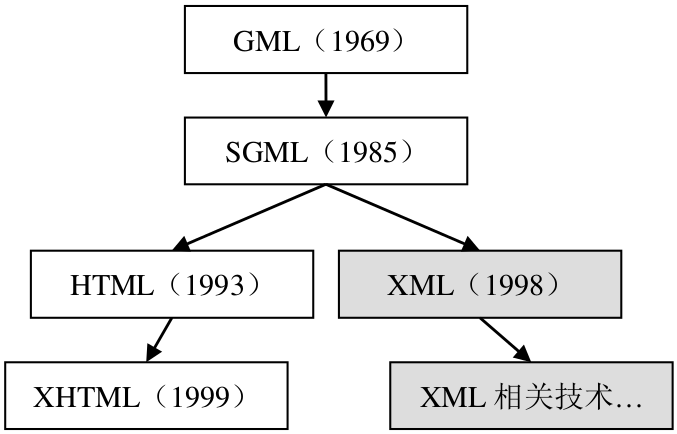
\includegraphics[width=0.8\textwidth]{figure/intro-1.png}
\end{figure}
\end{frame}


\subsection{1.2 XML 的设计目标与特点}


\begin{frame}{XML 的设计目标}
\begin{itemize} 
\item 可以直接应用于因特网
\item 支持各类不同的应用程序
\item 与 SGML 兼容
\item 处理 XML 文件的程序容易编写
\item 选择性功能的数量尽可能少
\item 清晰明了,可读性强
\item 设计应该合乎格式并且简洁
\item 容易创建
\item 标记必须保证其可读性,不能因为过于简化而导致含义模糊
\end{itemize}
\end{frame}


\begin{frame}{XML 的主要特点}
\begin{itemize} 
\item 具有良好的格式
\item 具有验证机制
\item 增强了 Web 应用的灵活性
\item 具有丰富的显示样式
\item 是电子数据交换 EDI 的通用格式
\item 支持复杂的数据关系和快捷的数据处理
\item 具有面向对象的特性
\item 是一种开放的标准
\item 技术体系性强
\end{itemize}

\par 思考XML的不足之处
\end{frame}


\subsection{1.3 XML 技术体系}
\begin{frame}[fragile]{ XML 技术体系}
\begin{figure}
	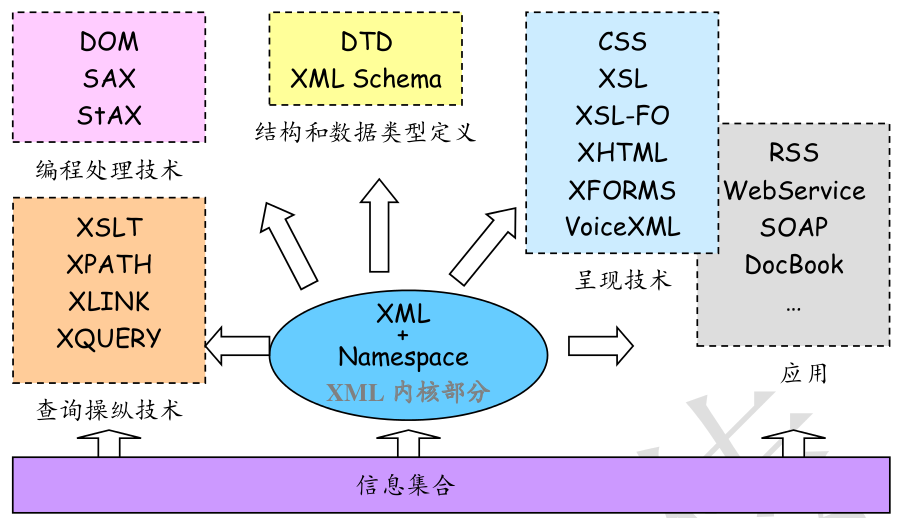
\includegraphics[width=0.8\textwidth]{figure/intro-2.png}
\end{figure}
\end{frame}


\subsection{1.4 XML 的应用与发展}
\begin{frame}[fragile]{ XML 的应用与发展}
\begin{itemize} 
\item 行业标记语言设计领域
\item 电子文件的长期保存领域
\item 电子数据交换领域
\item Web应用领域
\end{itemize}
\end{frame}


\subsection{1.5 XML 相关工具}
\begin{frame}[fragile]{ XML 相关工具}
\begin{itemize} 
\item 编辑工具:文本编辑工具、oXygen XML Editor、XML Spy \dots
\item 浏览工具:浏览器
\item 验证工具:浏览器、专用XML工具和软件包
\item 解析器:Apache Xerces
\end{itemize}
\end{frame}


\begin{frame}[fragile]{ oXygen XML Editor}
\begin{figure}
	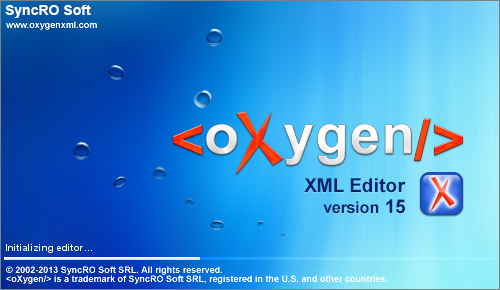
\includegraphics[width=0.8\textwidth]{figure/intro-oxygen.png}
\end{figure}
\begin{shaded}
\par 推荐使用,比XML Spy对标准的支持更好
\end{shaded}
\end{frame}


\begin{frame}[fragile]{ 教材}
\begin{center}
   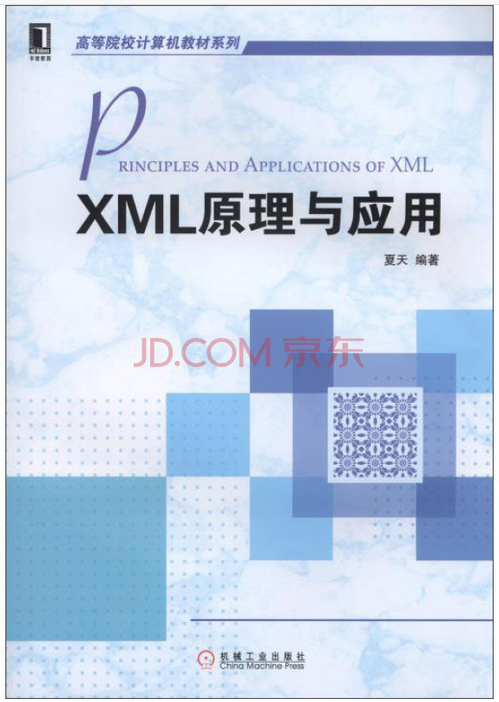
\includegraphics[width=0.4\textwidth]{figure/book-cover.png}
\end{center}
\end{frame}


\begin{frame}
\begin{center}
    \Huge END
\end{center}
\begin{figure}
    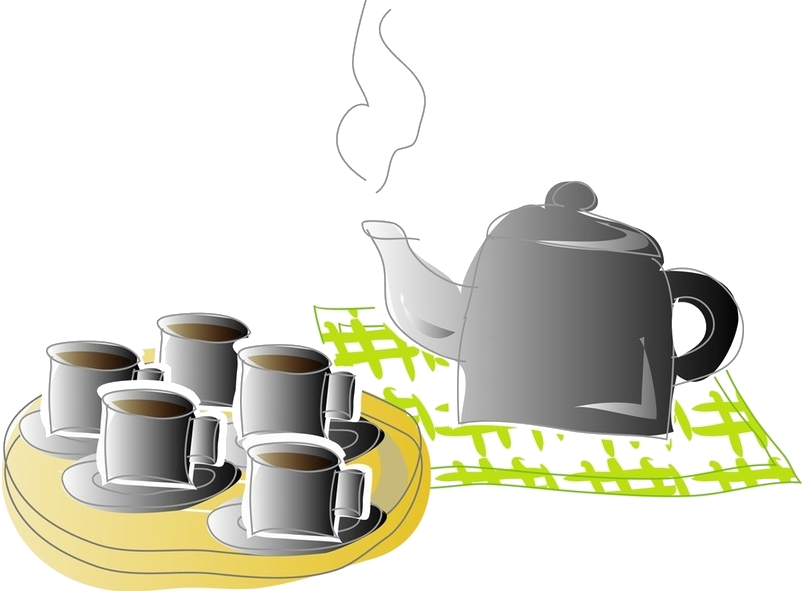
\includegraphics[width=0.75\textwidth]{figure/relax.png}
\end{figure}
\end{frame}
